\documentclass[15pt,a5paper,reqno]{article}
\usepackage{hyperref}
\usepackage[warn]{mathtext}
\usepackage[utf8]{inputenc}
\usepackage[T2A]{fontenc}
\usepackage[russian]{babel}
\usepackage{amssymb, amsmath, multicol}
\usepackage{graphicx}
\usepackage[shortcuts,cyremdash]{extdash}
\usepackage{wrapfig}
\usepackage{gensymb}
\usepackage{floatflt}
\usepackage{lipsum}
\usepackage{verbatim}
\usepackage{concmath}
\usepackage{euler}
\usepackage{xcolor}
\usepackage{etoolbox}
\usepackage{fancyhdr}
\usepackage{subfiles}
\usepackage{enumitem}
\usepackage{amsthm}
\usepackage{indentfirst}
\usepackage{import}
\usepackage{multirow}
\usepackage{hhline}
\usepackage{calrsfs}

\DeclareMathOperator{\sign}{sign}

\RequirePackage[ left     = 1cm,
                 right    = 1cm,
                 top      = 2.0cm,
                 bottom   = 1.25cm,
                 includefoot,
                 footskip = 1.25cm ]{geometry}
                 
\setlength{\parskip}{ .5em plus .15em minus .08em }
\renewcommand {\baselinestretch}{ 1.07 }

\fancyhf{} % clear existing header/footer entries

\renewcommand{\footrulewidth}{ .0em }
\fancyfoot[C]{\texttt{\textemdash~\thepage~\textemdash}}

\makeatletter
\patchcmd\l@section{%
  \nobreak\hfil\nobreak
}{%
  \nobreak
  \leaders\hbox{%
    $\m@th \mkern \@dotsep mu\hbox{.}\mkern \@dotsep mu$%
  }%
  \hfill
  \nobreak
}{}{\errmessage{\noexpand\l@section could not be patched}}
\makeatother
\parindent = 1cm % отступ при красной строке⏎
\pagestyle{fancy}    
\renewcommand\qedsymbol{$\blacksquare$}

\newcommand{\when}[2]{
  \left. #1 \right|_{#2} \hspace
}
\renewcommand{\kappa}{\varkappa}
\RequirePackage{caption2}
\renewcommand\captionlabeldelim{}
\newcommand*{\hm}[1]{#1\nobreak\discretionary{}

\DeclareSymbolFont{T2Aletters}{T2A}{cmr}{m}{it}
{\hbox{$\mathsurround=0pt #1$}}{}}
% Цвета для гиперссылок
\definecolor{linkcolor}{HTML}{000000} % цвет ссылок
\definecolor{urlcolor}{HTML}{799B03} % цвет гиперссылок
 
\hypersetup{pdfstartview=FitH,  linkcolor=linkcolor,urlcolor=urlcolor, colorlinks=true}


\begin{document}

% НАЧАЛО ТИТУЛЬНОГО ЛИСТА
\begin{center}
  {\small ФЕДЕРАЛЬНОЕ ГОСУДАРСТВЕННОЕ АВТОНОМНОЕ ОБРАЗОВАТЕЛЬНОЕ\\ УЧРЕЖДЕНИЕ ВЫСШЕГО ОБРАЗОВАНИЯ\\ МОСКОВСКИЙ ФИЗИКО-ТЕХНИЧЕСКИЙ ИНСТИТУТ\\ (НАЦИОНАЛЬНЫЙ ИССЛЕДОВАТЕЛЬСКИЙ УНИВЕРСИТЕТ)\\ ФИЗТЕХ-ШКОЛА РАДИОТЕХНИКИ И КОМПЬЮТЕРНЫХ ТЕХНОЛОГИЙ}\\
  \hfill \break
  \hfill \break
  \hfill \break
  \Huge{Работа 3.3.5. \\ Эффект Холла в металлах}\\
\end{center}

\hfill \break
\hfill \break
\hfill \break
\hfill \break
\hfill \break
\hfill \break
\hfill \break
\hfill \break
\hfill \break
\hfill \break
\hfill \break
\hfill \break
\hfill \break

\begin{flushright}
  \normalsize{Работу выполнил:}\\
  \normalsize{\textbf{Долгов Александр Алексеевич, группа Б01-106}}\\
\end{flushright}

\begin{center}
  \normalsize{\textbf{Долгопрудный, 2022}}
\end{center}

\thispagestyle{empty} % выключаем отображение номера для этой страницы

% КОНЕЦ ТИТУЛЬНОГО ЛИСТА

\newpage
\thispagestyle{plain}
\tableofcontents
\thispagestyle{plain}
\newpage

\section{Аннотация}

    В работе изучаются особенности проводимости металлов в геометрии мостика Холла. Ток пропускается по плоской прямоугольной металлической пластинке, помещённой в перпендикулярное пластинке магнитное поле. Измеряется разность потенциалов между краями пластинки в поперечном к току направлении. По измерениям определяется константа Холла, тип проводимости (электронный или дырочный) и вычисляется концентрация основных носителей заряда.
    
\section{Теоретические сведения}

    На заряд в электромагнитном поле действует сила Лоренца:
    \begin{equation}
        \vec{F} = q\vec{E} + q[\vec{v}, \vec{B}]
    \end{equation}
    Эта сила вызывает движение носителей, направление которого в общем случае не совпадает с $\vec{E}$. Отклонившиеся носители скапливаются на поверхности проводника так, что образуют электрическое поле, компенсирующее внешнее магнитное поле. Возникновение поперечного току электрического поля в образце, помещённом в магнитном поле, называют \textit{эффектом Холла}.

    
    Закон Ома в дифференциальной форме:
    \begin{equation*}
        \vec{j} = \widehat{\sigma}\vec{E},\text{ где } \widehat{\sigma} = 
        \begin{pmatrix}
            \sigma_{xx} & \sigma_{xy} & \sigma_{xz} \\
            \sigma_{yx} & \sigma_{yy} & \sigma_{yz} \\
            \sigma_{xz} & \sigma_{zy} & \sigma_{zz}
        \end{pmatrix}
        \text{ - тензор проводимости}
    \end{equation*}
    Пусть система содержит носители заряда только одного типа. Индукцию магнитного поля $\vec{B}$ направим вдоль оси Oz. Так как ток постоянный, то заряды движутся в среднем с постоянной скоростью $\implies$ сила Лоренца уравновешена "трением"\ со стороны среды:
    \begin{equation*}
        q(\vec{E} + [\vec{v}, \vec{B}]) - \frac{q\vec{v}}{\mu} = 0
    \end{equation*}
    \begin{equation*}
        \vec{E} = \frac{\vec{v}}{\mu} - [\vec{v}, \vec{B}]
    \end{equation*}
    Связь плотности тока со средней скоростью носителей заряда:
    \begin{equation*}
        \vec{j} = qn\vec{v} \implies \vec{v} = \frac{\vec{j}}{qn}
    \end{equation*}
    Следовательно:
    \begin{equation*}
        \vec{E} = \frac{\vec{j}}{qn\mu} - \frac{1}{qn}[\vec{j}, \vec{B}]
    \end{equation*}
    Введём обозначение: $\sigma_0 = qn\mu$ - удельная проводимость среды в отсутствии магнитного поля. С учётом этого обозначения формула примет окончательный вид:
    \begin{equation}\label{vec_E}
        \boxed{\vec{E} = \frac{\vec{j}}{\sigma_0} - \frac{1}{qn}[\vec{j}, \vec{B}]}
    \end{equation}
    Последнее равенство можно записать в проекциях на координатные оси:
    \begin{equation*}
        E_x = \frac{j_x}{\sigma_0} - \frac{j_yB}{nq};\ E_y = \frac{j_y}{\sigma_0} + \frac{j_xB}{nq};\ E_z = \frac{j_z}{\sigma_0}
    \end{equation*}
    Соответственно, соотношение \eqref{vec_E} может быть записано в матричном виде:
    \begin{equation}\label{resistance_tensor}
        \vec{E} =
        \begin{pmatrix}
            1 & -\mu B & 0 \\
            \mu B & 1 & 0 \\
            0 & 0 & 1
        \end{pmatrix}
        \frac{\vec{j}}{\sigma_0}
    \end{equation}
    Матрицу тензора проводимости находим как обратную к матрице в уравнении \eqref{resistance_tensor}:
    \begin{equation}\label{conductivity_tensor}
    \boxed{\widehat{\sigma} = \frac{\sigma_0}{1 + (\mu B)^2}
            \begin{pmatrix}
                1 & \mu B & 0 \\
                -\mu B & 1 & 0 \\
                0 & 0 & 1
            \end{pmatrix}}
    \end{equation}
    Безразмерный коэффициент $\mu B$ называется \textit{параметром замагниченности}.

    Для исследования зависимости проводимости среды от магнитного поля используется мостик Холла (см. рис 2) В данной схеме ток вынуждают течь по оси $Ox$ вдоль плоской пластинки (ширина пластинки $a$, толщина $h$, длина $l$). 
    \begin{center}
        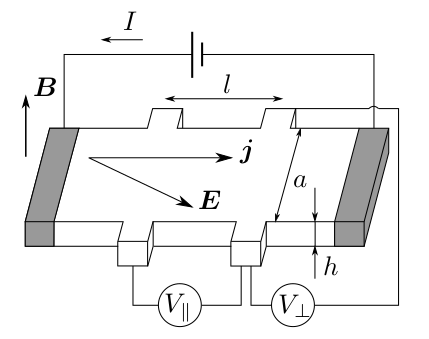
\includegraphics[width = 0.5\textwidth]{images/picture_2.png}\\
        \textbf{Рисунок 2. Мостик Холла}
    \end{center}
    В проводимом опыте мостик имел следующие параметры:\\
    \textbf{Медь}: h = 0.05 мм, $l_{34}$ = 6 мм l = 8 мм\\
    \textbf{Цинк}: h = 0.12 мм, $l_{34}$ = 3.5 мм, l = 10.5 мм\\
    
    Сила Лоренца, действующая со стороны перпендикулярного пластинке магнитного поля, «прибивает» носители заряда к краям образца, что создаёт холловское электрическое поле, компенсирующее эту силу. Поперечное напряжение между краями пластинки (холловское напряжение) равно $U_{\perp} = E_ya$, где:
    \begin{equation*}
        E_y = \frac{j_x B}{nq}
    \end{equation*}
    Плотность тока, текущего через образец, равна $j_x = I/ah$, где $I$ — полный ток. Таким образом, для холловского напряжения имеем
    \begin{equation}\label{holes_voltage}
        \boxed{U_{\perp} = \frac{B}{nqh}I = R_H I \frac{B}{h}}
    \end{equation}
    Константу $R_H = 1/nq$ называют \textit{постоянной Холла}. Знак постоянной Холла определяется знаком заряда носителей. Продольная напряжённость электрического поля равна
    \begin{equation*}
        E_x = j_x / \sigma_0
    \end{equation*}
    и падение напряжения $U_{||} = E_x l$ вдоль пластинки определяется омическим сопротивлением образца $R_0 = l / (\sigma_0 a h)$:
    \begin{equation*}
        U_{||} = IR_0
    \end{equation*}
    Интересно отметить, что несмотря на то, что тензор проводимости (3.26) явно зависит от $B$, продольное сопротивление образца в данной геометрии от магнитного поля не зависит.

\section{Экспериментальная установка}

    \begin{center}
        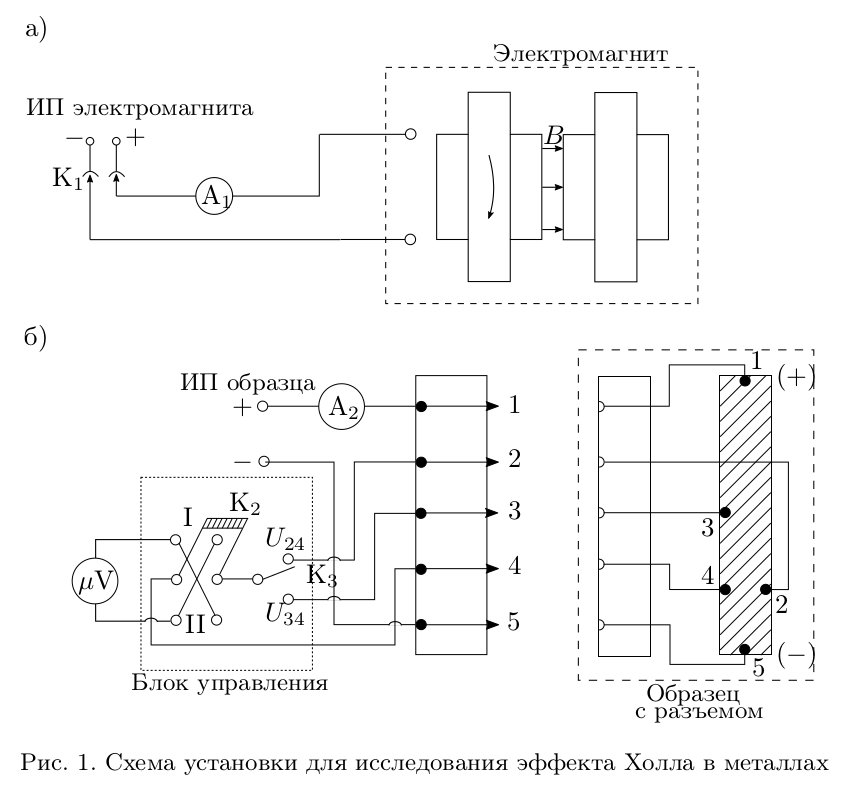
\includegraphics[width=0.7\textwidth]{images/picture_1.png}
    \end{center}
    \noindentЭлектрическая схема установки для измерения ЭДС Холла представлена на рис. 1. В зазоре электромагнита (рис. 1а) создаётся постоянное магнитное поле, величину которого можно менять с помощью источника питания электромагнита. Разъём $K_1$ позволяет менять направление тока в обмотках электромагнита. Ток питания электромагнита измеряется амперметром $A_1$. Градуировка электромагнита (связь тока с индукцией поля) проводится при помощи миллитесламетра на основе датчика Холла. Металлические образцы в форме тонких пластинок, смонтированные в специальных держателях, подключаются к блоку питания через разъём (рис. 1б). Ток через образец регулируется реостатом $R_2$ и измеряется амперметром $A_2$.
    
    В образце с током, помещённом в зазор электромагнита, между контактами 2 и 4 возникает холловская разность потенциалов $U_{\perp}$, которая измеряется с помощью микровольтметра, если переключатель $K_3$ подключён к точке 2 образца. При подключении $K_3$ к точке 3 микровольтметр измеряет омическое падение напряжения $U_{34}$ , вызванное током через образец. При нейтральном положении ключа входная цепь микровольтметра разомкнута. Ключ $K_2$ позволяет менять полярность напряжения, поступающего на вход микровольтметра.

    \section{Методика измерений}
    
    Контакты 2 и 4 вследствие неточности подпайки могут лежать не на одной эквипотенциали. Тогда напряжение между ними связано не только с эффектом Холла, но и с омическим падением напряжения вдоль пластинки. Исключить этот эффект можно, если при каждом значении тока через образец измерять напряжение между точками 3 и 4 в отсутствие магнитного поля. При фиксированном токе через образец это дополнительное к ЭДС Холла напряжение $U_0$ остаётся неизменным. От него следует (с учётом знака) отсчитывать величину ЭДС Холла:
    \begin{equation*}
        U_{\perp} = U_{24} - U_0
    \end{equation*}
    По знаку $U_{\perp}$ можно определить характер проводимости — электронный или дырочный. Для этого необходимо знать направление тока в образце и направление магнитного поля.

    Измерив ток $I$ в образце и напряжение $U_{34}$ между контактами 3 и 4
    в отсутствие магнитного поля, можно, зная параметры образца, рассчитать удельное сопротивление $\rho_0$ и проводимость $\sigma_0$ материала образца по формуле
    \begin{equation}\label{rho}
        \boxed{\rho_0 = \frac{U_{34}ah}{Il}},
    \end{equation}
    где $l$ — расстояние между контактами 3 и 4.

\section{Измерения и обработка их результатов}

    \subsection{Калибровочная кривая электромагнита}
        Сначала была проведена калибровка электромагнита. Её результаты приведены в \hyperlink{table_1}{Таблице 1}.

    \subsection{Находжение постоянной Холла для медного образца}
        Была измерена зависимость напряжения $U_{24}$ между контактами 2 и 4 от тока через электромагнит при различных токах через образец. Всего было проведено 5 серий измерений, результаты которых представлены в \hyperlink{table_2}{Таблице 2}. По данным этой таблицы и с помощью найденной калибровочной кривой построена зависимость ЭДС Холла от индукции магнитного поля между полюсами электромагнита при каждом из значений тока через образец. Графики 1-5 иллюстрируют эту зависимость.

        Угловые коэффициенты аппроксимирующих прямых сведены в \hyperlink{table_3}{Таблицу 3}. По данным этой таблицы построен график зависимости угловых коэффициентов от тока через образец: \hyperlink{graph_6}{График 6}. По этому графику возможно найти постоянную Холла:
        \begin{equation*}
            R_H = hk_2,
        \end{equation*}
        где $k_2$ - угловой коэффициент прямой на графике 6.
        Имеем:
        \begin{equation*}
            R_H = 1.41\cdot 10^{-6}\frac{\text{В}}{\text{Тл}\cdot\text{А}} \cdot 5 \cdot 10^{-5} м = 7.05 \cdot 10^{-11}\frac{\text{м}^3}{\text{Кл}}
        \end{equation*}

    \subsection{Определение концентрация носителей}

        Так как в металлах свободными носителями заряда являются электроны, то их концентрацию можно найти по формуле
        \begin{equation*}
            n = \frac{1}{eR_H}
        \end{equation*}
        Для меди получаем:
        \begin{equation*}
            n_{Cu} = \frac{1}{1.6 \cdot 10^{-19}\text{ Кл}\cdot 7.05 \cdot 10^{-11}\frac{\text{м}^3}{\text{Кл}}} = 8.9\cdot 10^{28}\text{м}^3
        \end{equation*}

    \subsection{Определение удельной проводимости}

        Было проведено по одному измерению напряжения между контактами 3 и 4 и тока через образец в отсутствии магнитного поля для меди и цинка. Результаты представлены в \hyperlink{table_4}{Таблице 4}.
        
        Согласно \eqref{rho} 
    
\section{Вывод}

    
    
\newpage
\section{Приложения}

    \subsection{Таблицы}

    \noindent\hypertarget{table_1}{\textbf{Таблица 1. Калибровка электромагнита}}
    \begin{center}
        \begin{tabular}{|c|c|}
            \hline
            I, A & B, мТл \\ \hline\hline
            0    & 16.37  \\ \hline
            0.16 & 169.5  \\ \hline
            0.32 &  332   \\ \hline
            0.48 &  492   \\ \hline
            0.64 &  655   \\ \hline
            0.80 &  774   \\ \hline
            0.96 &  857   \\ \hline
            1.12 &  920   \\ \hline
            1.28 &  971   \\ \hline   
        \end{tabular}
    \end{center}

    \noindent\hypertarget{table_2}{\textbf{Таблица 2. Измерения ЭДС Холла}}
    \begin{center}
        \begin{tabular}{|c|c|c|c|c|c|}
            \hline
            \multicolumn{2}{|c|}{I = 0.2 A} & \multicolumn{2}{|c|}{I = 0.4 A} & \multicolumn{2}{|c|}{I = 0.6 A} \\ \hline
            \multicolumn{2}{|c|}{$U_0$ = 0.08 мкВ} & \multicolumn{2}{|c|}{$U_0$ = 0.12 мкВ} & \multicolumn{2}{|c|}{$U_0$ = 0.2 мкВ} \\ \hline\hline 
            $I_M$, A & $U_{24}$, мкВ & $I_M$, A & $U_{24}$, мкВ & $I_M$, A & $U_{24}$, мкВ \\ \hline\hline
            0.16     & 0.16   & 0.16     & 0.24   & 0.16     & 0.28   \\ \hline
            0.32     & 0.2    & 0.32     & 0.32   & 0.32     & 0.44   \\ \hline
            0.48     & 0.24   & 0.48     & 0.4    & 0.48     & 0.56   \\ \hline
            0.64     & 0.28   & 0.64     & 0.52   & 0.64     & 0.72   \\ \hline
            0.8	     & 0.32   & 0.8      & 0.6    & 0.8      & 0.8    \\ \hline
            0.96     & 0.356  & 0.96     & 0.64   & 0.96     & 0.88   \\ \hline
            1.12     & 0.364  & 1.12     & 0.64   & 1.12     & 0.96   \\ \hline
            1.26     & 0.38   & 1.23     & 0.66   & 1.23     & 0.96   \\ \hline
        \end{tabular}
    \end{center}
    \begin{center}
        \begin{tabular}{|c|c|c|c|}
            \hline
            \multicolumn{2}{|c|}{I = 0.8 A} & \multicolumn{2}{|c|}{I = 1 A} \\ \hline
            \multicolumn{2}{|c|}{$U_0$ = 0.2 мкВ} & \multicolumn{2}{|c|}{$U_0$ = 0.28 мкВ} \\ \hline\hline
            $I_M$, A & $U_{24}$, мкВ & $I_M$, A & $U_{24}$, мкВ \\ \hline\hline
            0.16     & 0.36   & 0.16     & 0.48   \\ \hline
            0.32     & 0.56   & 0.32     & 0.72   \\ \hline
            0.48     & 0.76   & 0.48     & 0.96   \\ \hline
            0.64     & 0.96   & 0.64     & 1.16   \\ \hline
            0.8      & 1.08   & 0.8      & 1.36   \\ \hline
            0.96     & 1.16   & 0.96     & 1.44   \\ \hline
            1.12     & 1.24   & 1.12     & 1.52   \\ \hline
            1.22     & 1.28   & 1.22     & 1.6    \\ \hline
        \end{tabular}
    \end{center}

    \noindent\hypertarget{table_3}{\textbf{Таблица 3. Угловые коэффициенты аппроксимирующих прямых}}
    \begin{center}
        \begin{tabular}{|c|c|}
             \hline
             I, A & k, $10^{-6}\frac{\text{В}}{\text{Тл}}$ \\ \hline\hline
             0.2 & 0.279 \\ \hline
             0.4 & 0.556 \\ \hline
             0.6 & 0.863 \\ \hline
             0.8 & 1.152 \\ \hline
             1.0 & 1.386 \\ \hline
        \end{tabular}
    \end{center}

    \noindent\hypertarget{table_3}{\textbf{Таблица 4. Определение удельной проводимости}}
    \begin{center}
        \begin{tabular}{|c|c|c|}
            \hline
                   & Медь & Цинк \\ \hline
            I, A   &  1   & 1    \\ \hline
            U, мкВ & 320  & 380  \\ \hline 
        \end{tabular}
    \end{center}

    \newpage
    \subsection{Графики}

    \noindent\hypertarget{graph_1}{\textbf{График 1. I = 0.2 A}}
    \begin{center}
        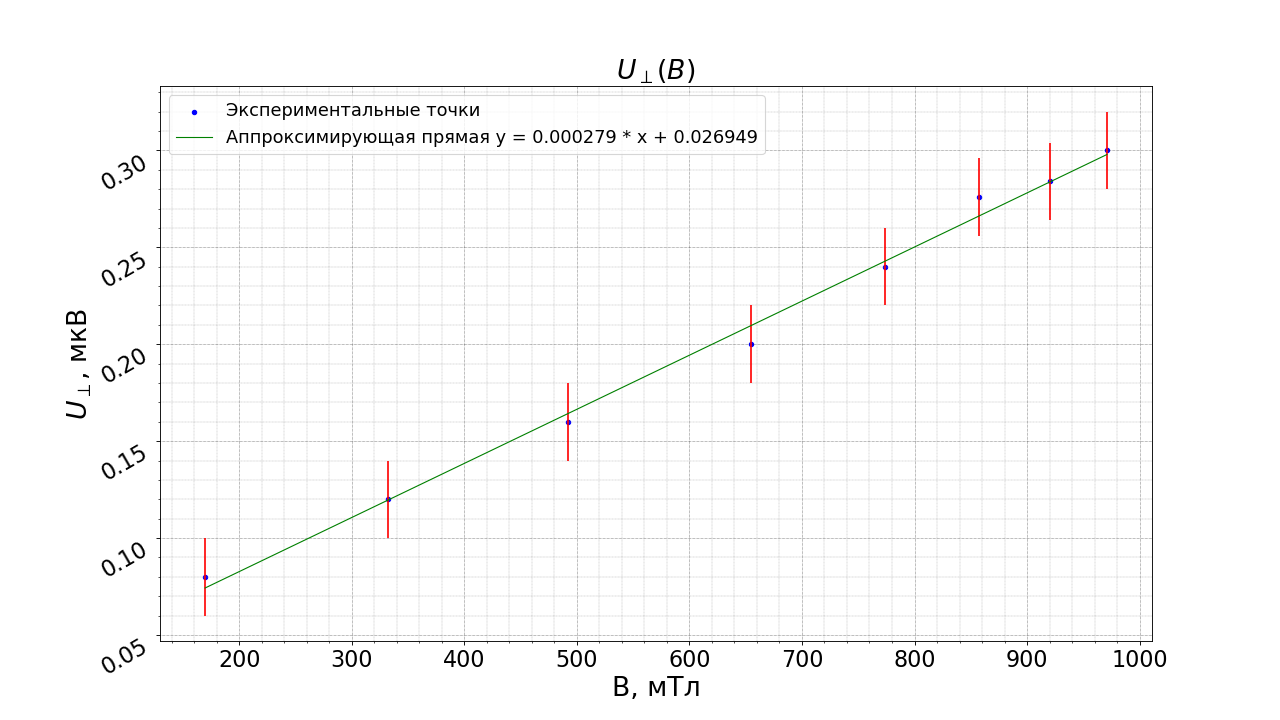
\includegraphics[width = 0.9\textwidth]{images/graph_1.png}
    \end{center}

    \noindent\hypertarget{graph_2}{\textbf{График 2. I = 0.4 A}}
    \begin{center}
        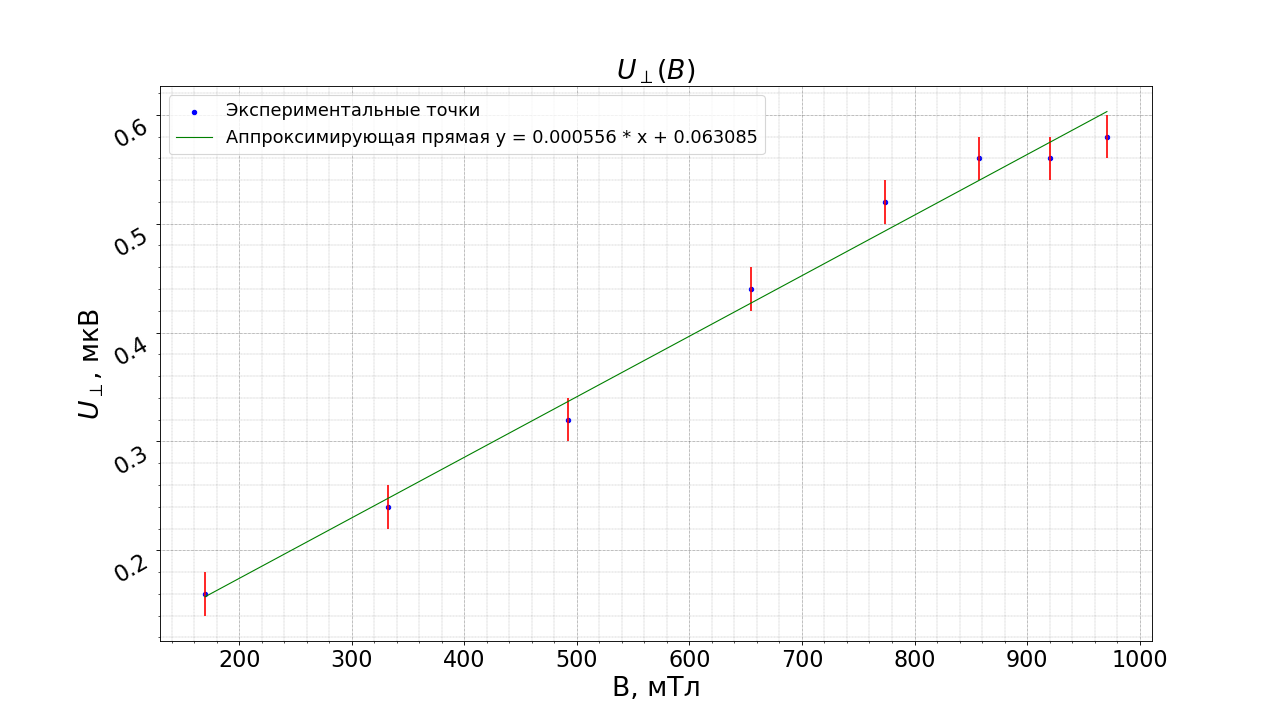
\includegraphics[width = 0.9\textwidth]{images/graph_2.png}
    \end{center}

    \noindent\hypertarget{graph_3}{\textbf{График 3. I = 0.6 A}}
    \begin{center}
        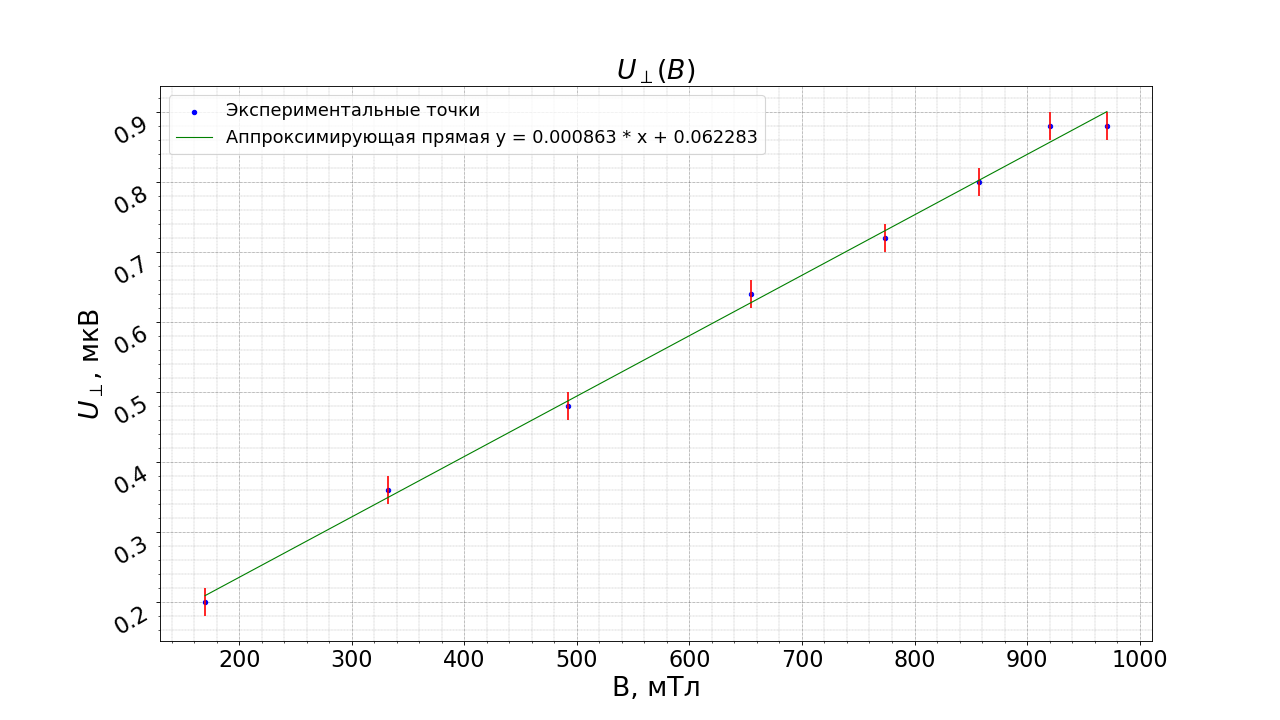
\includegraphics[width = \textwidth]{images/graph_3.png}
    \end{center}

    \noindent\hypertarget{graph_4}{\textbf{График 4. I = 0.8 A}}
    \begin{center}
        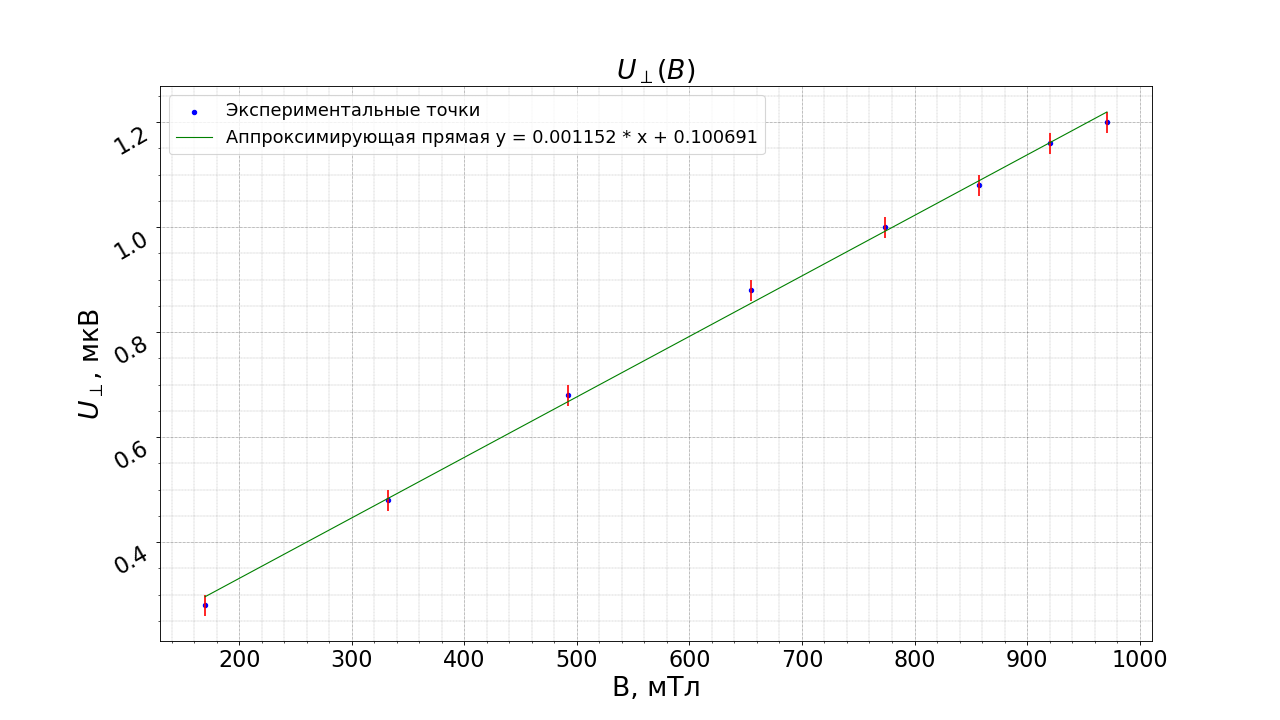
\includegraphics[width = \textwidth]{images/graph_4.png}
    \end{center}

    \noindent\hypertarget{graph_5}{\textbf{График 5. I = 1 A}}
    \begin{center}
        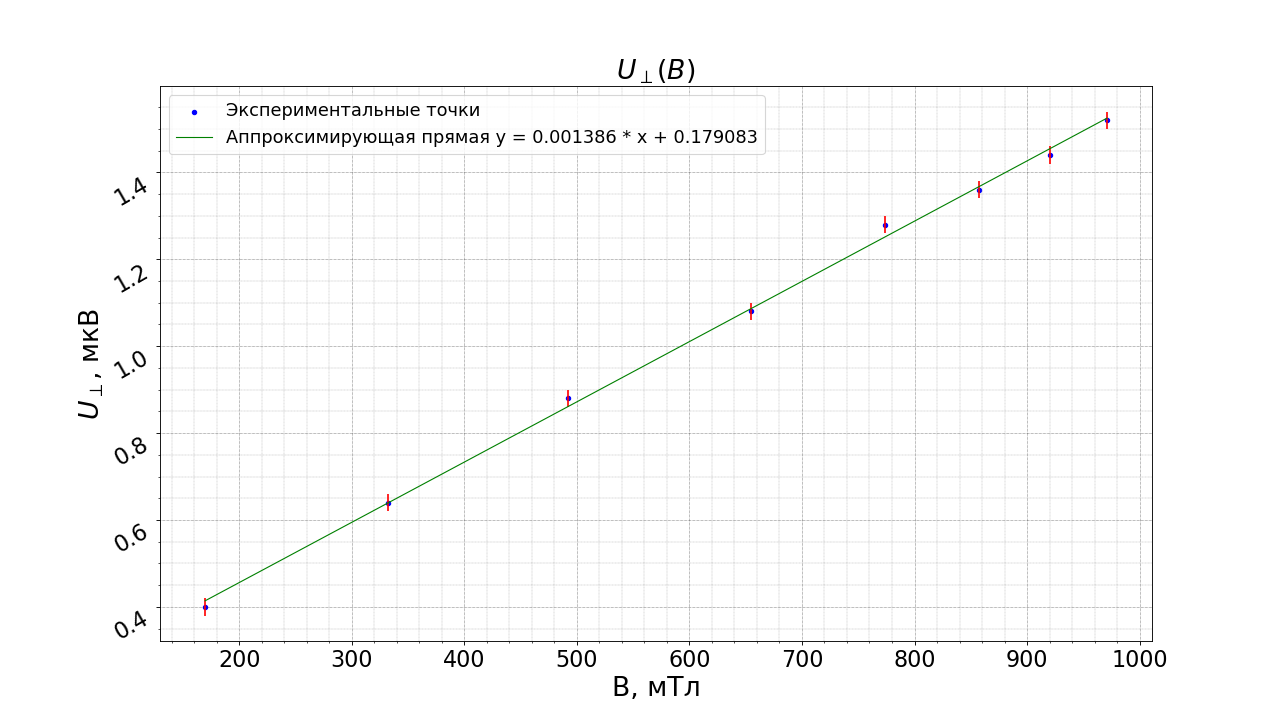
\includegraphics[width = \textwidth]{images/graph_5.png}
    \end{center}

    \noindent\hypertarget{graph_6}{\textbf{График 6. k(I)}}
    \begin{center}
        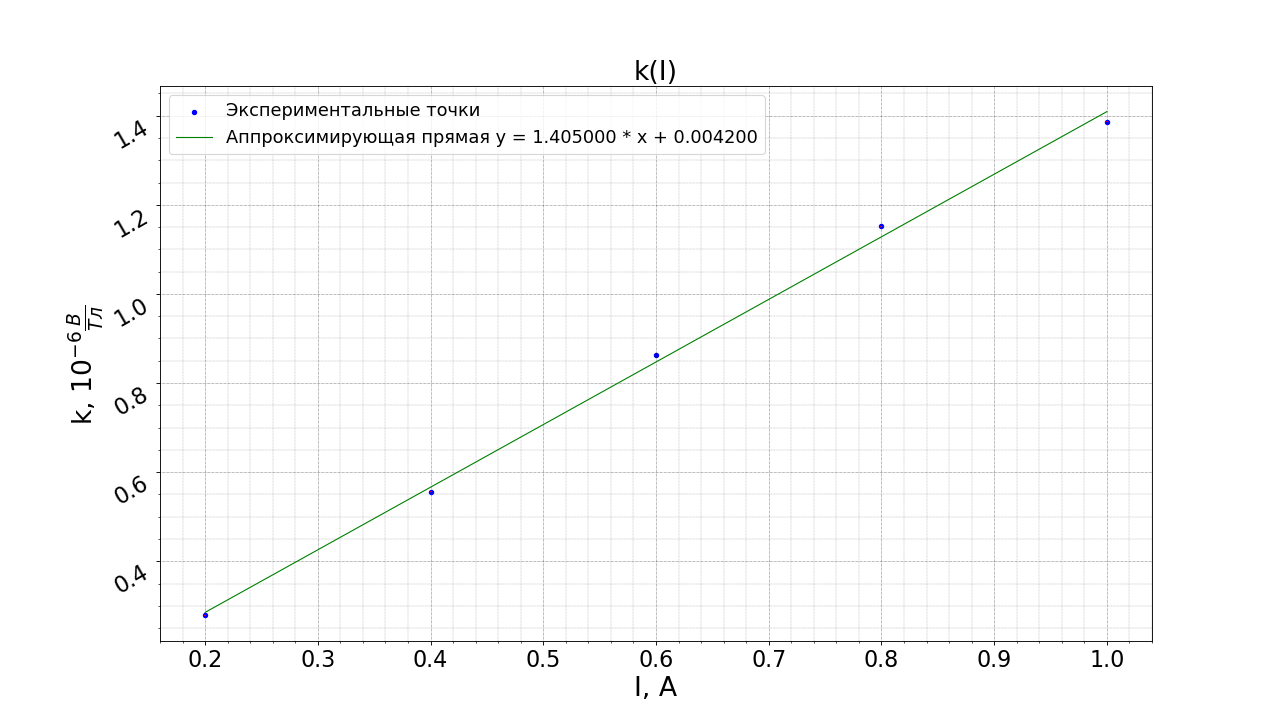
\includegraphics[width = \textwidth]{images/graph_6.png}
    \end{center}

\end{document}
